%%% Local Variables:
%%% mode: latex
%%% TeX-master: t
%%% End:
\chapter{基于模式解耦的弹性波最小平方逆时偏移}
\label{cha:MD-ELSRTM}
\section{引言}
前一章内容中我们将模型分解为高波数与低波数成分,并通过弹性波WERTI方式来恢复模型的低波数成分。常规的FWI算法可以恢复模型的高波数成分,但是会受到许多因素干扰,
如cycle-skipping问题,信噪比低,地震子波未知,正演算子不准确等等。除此之外,我们通常也会通过最小平方偏移(LSM)来实现高波数成分的重构。
早在1993年,Schuster(1993)\cite{Schuster1993}提出了针对井间数据的LSM算法,而Nemeth et al.\cite{Nemeth1999}将该方法应用到了地面数据中。
以波动方程为引擎的最小平方逆时偏移(LSRTM)近年来一直是研究的热点,例如Dai and
Schuster(2013)\cite{Dai2013},Dong et al.(2012)\cite{Dong2012}, Luo and
Hale(2014)\cite{Luo2014}。尽管其计算代价昂贵,但是LSRTM可以回避模型速度复杂时所产生的多路径问题。
LSRTM的过程通常被认为是线性的全波形反演,其假设在已经获得足够好的低波数模型成分之后恢复模型的高频扰动,也即获得“像”,使得在最小平方意义下,
用该“像”所预测的反射数据能与观测数据达到最佳匹配。因此,最小平方逆时偏移与全波形反演的理论框架是一致的。

近期,为了更准确地描述波传播过程,同时获得更多的参数
成像,并解决多参数带来的耦合效应,原本基于声波方程的
LSRTM被推广到了变密度声波介质\cite{Yang2017},衰减介质\cite{Dai2015}以及弹性介质中\cite{Duan2016,Feng2016,Xu2016}(ELSRTM)。
相比声波成像,弹性波成像可以提供更多的地下信息,例如裂缝分布以及弹性性质。但是,弹性波偏移中存在的许多问题会很大程度上影响成像质量。因为通常很难将记录中的
波模式完全区分开,因此其中某些波模式的会因速度不对而被错误地成像。这些非物理的模式就会引起假象,也即“cross-talk”。
而通过ELSRTM则可以提高成像的分辨率,并且可以压制由于观测孔径限制,粗网格采样以及数据缺失引起的偏移假象。
弹性波成像需要处理矢量波的问题,也就需要选取合适的成像条件,{\color{red}\cite{Wang2016}提出了无极性反转的矢量成像条件等等。}而从EFWI理论框架出发,许多学者,
如Duan et al.(2016)\cite{Duan2016},Feng et
al.(2016)\cite{Feng2016}等都推导出了与EFWI梯度非常类似的成像条件。该成像条件也可以回避极性反转问题,同时也可以认为是更加接近于高频的参数扰动梯度。而基于
第二章中对EFWI算法的分析,模式解耦带来的优势将同样能在ELSRTM中得以应用,因此我们将在本章中应用波模式解耦来对ELSRTM进行预条件,从而获得更好结果。
\section{弹性}
假设在背景弹性介质$c_{ijkl}$中有一个参数扰动$\delta c_{ijkl}$,则背景波场与扰动波场满足以下方程:
\begin{equation}
    \rho \frac{\partial u^2_i}{\partial t^2}  -
    \frac{\partial}{\partial x_j}\left[ 
        c_{ijkl}\frac{\partial u_{k}}{\partial
        x_l}\right]=f_i,
    \label{eq:WE} 
\end{equation}
和
\begin{equation}
    \rho \frac{\partial \delta u^2_i}{\partial t^2}  -
    \frac{\partial}{\partial x_j}\left[ 
        c_{ijkl}\frac{\partial \delta u_{k}}{\partial
        x_l}\right]=\frac{\partial}{\partial x_j}\left[\delta c_{ijkl}\frac{\partial u_{k}}{\partial x_l}\right],
    \label{eq:DeltaWE} 
\end{equation}
其中,$\delta u_i$可以看作是用RTM或其他方法的成像结果,$\delta c_{ijkl}$进行反偏移之后的反射数据。在WERTI中,我们需要使得观测数据$\mathbf{d}^{o}$与模拟数据
$\mathbf{d}^{c}$之间的走时残差最小,则目标函数为:
\begin{equation}
    E=\frac{1}{2}\int\tau^2(\mathbf{x_r},t;\mathbf{x_s})dtd\mathbf{x_r}d\mathbf{x_s},
    \label{eq:Objectivefunction} 
\end{equation}
其中,走时残差$\tau(\mathbf{x_r},t;\mathbf{x_s})$可以通过DIW来获取。通过类似Ma and
Hale (2013)\cite{Ma2013}的推导(见附录\ref{cha:AdjointForEWERTI}),我们可以得到如下梯度公式:
\begin{equation}
    \frac{\partial E}{\partial c_{ijkl}}=-\int (\frac{\partial u_{i}}{\partial
    x_j}\frac{\partial \delta \psi_{k}}{\partial x_l}+\frac{\partial \delta u_{i}}{\partial
    x_j}\frac{\partial \psi_{k}}{\partial x_l}),
    \label{eq:GradientCijkl}
\end{equation}
其中,$\psi_i$和$\delta \psi_i$是共轭波场满足:
\begin{equation}
    \rho \frac{\partial \psi^2_i}{\partial t^2}  -
    \frac{\partial}{\partial x_j}\left[ 
        c_{ijkl}\frac{\partial \psi_{k}}{\partial
        x_l}\right]=\tau(\mathbf{x_r},t;\mathbf{x_s})\frac{\dot{d}^o_i(\mathbf{x_r},t+\tau;\mathbf{x_s})}{h_i(\mathbf{x_r},t;\mathbf{x_s})},
    \label{eq:AdjointWE} 
\end{equation}
和
\begin{equation}
    \rho \frac{\partial \delta \psi^2_i}{\partial t^2}  -
    \frac{\partial}{\partial x_j}\left[ 
        c_{ijkl}\frac{\partial \delta \psi_{k}}{\partial 
        x_l}\right]=\frac{\partial}{\partial x_j}\left[\delta c_{ijkl}\frac{\partial
        \psi_{k}}{\partial x_l}\right], 
    \label{eq:AdjointDeltaWE} 
\end{equation}
上式中$h_i(\mathbf{x_r},t;\mathbf{x_s})=(\dot{d}^o_i(\mathbf{x_r},t+\tau;\mathbf{x_s}))^2-\ddot{d}^o_i(\mathbf{x_r},t+\tau;\mathbf{x_s})
(d^c_i(\mathbf{x_r},t;\mathbf{x_s})-d^o_i(\mathbf{x_r},t+\tau;\mathbf{x_s}))$,而$\dot{d}$则代表$d$在时间方向的导数。在方程\eqref{eq:GradientCijkl}的右端项
中,第一和第二项分别表示震源端和检波点端的反射波路径。之后我们可以通过链式法则来导出P波与S波速度的梯度公式:
\begin{equation}
    \frac{\partial E}{\partial V_p}=2\rho V_p\frac{\partial E}{\partial
        c_{ijkl}}\delta_{ij}\delta_{kl}, \qquad
    \frac{\partial E}{\partial V_s}=2\rho V_s\frac{\partial
    E}{\partial c_{ijkl}}(-2\delta_{ij}\delta_{kl}+\delta_{ik}\delta_{jl}+
    \delta_{il}\delta_{jk}).
    \label{eq:GradientVel}
\end{equation}
\section{弹性波WERTI工作流程}
弹性波介质中,不同模式的转换波,主要是PP与PS同相轴之间,会互相叠加、互相交叉。在用DIW提取走时差的时候,这些交叉点的位置就会变成一些奇异点而给拾取带来很大困难
。因此,如果直接用原始多分量数据的话,拾取到的$\tau(\mathbf{x_r},t;\mathbf{x_s})$就会不准确,这也是为什么式\eqref{eq:AdjointDeltaWE}中的梯度很难直接应用。
为了解决这个问题,我们将观测与模拟地震数据分解为P波与S波两部分。该模式分解只作用于地面地震数据\cite[]{Li2016a},因此我们可以快速地获得每一炮数据分解之后的矢量
P波或S波地震记录。这样,走时残差就可以被分成P波与S波两部分,使得弹性波WERTI变得可行,也即用一个两阶段的流程,先P波阶段后S波阶段。

在P波阶段,主要采用PP反射波来建立P波速度的背景模型。首先,我们从ERTM中获得P波速度的扰动,也即$\delta V_p$。由于在WERTI中我们只考虑走时,所以我们只进行ERTM成像
而不是最小平方ERTM来拟合反射波振幅。因此,目标函数可以变做最小化PP反射波的走时残差:
\begin{equation}
    E_{pp}=\frac{1}{2}\int\tau^2_{pp}(\mathbf{x_r},t;\mathbf{x_s})dtd\mathbf{x_r}d\mathbf{x_s}.
    \label{eq:ObjectivefunctionPP} 
\end{equation}
这样,采用P波记录来计算方程\eqref{eq:AdjointWE}的右端项,并用$\delta V_p$替换方程\eqref{eq:DeltaWE}和\eqref{eq:AdjointDeltaWE}中的$\delta c_{ijkl}$,我们
就可以计算得到$V_p$的梯度, $\frac{\partial E}{\partial V_p}$。

在S波阶段,我们将采用类似的策略但是只利用PS反射波。则目标函数变为:
\begin{equation}
    E_{ps}=\frac{1}{2}\int\tau^2_{ps}(\mathbf{x_r},t;\mathbf{x_s})dtd\mathbf{x_r}d\mathbf{x_s}.
    \label{eq:ObjectivefunctionPS} 
\end{equation}
但是,实现方式与前一阶段策略略有不同。经过P波阶段反演之后,$V_p$的背景速度已经获得了很好的恢复,此时PP波成像结果应该已经比较接近准确位置。而通常情况下,地
下介质中$V_p$与$V_s$的界面是比较一致的。所以,我们推荐采用较为准确的PP成像($\delta V_p$)结果而不是$\delta V_s$来产生PS反射波。此外,在PS反射中,波路径的
震源端只与P波速度相关,因此我们在计算$\frac{\partial E}{\partial V_s}$可以丢掉方程\eqref{eq:GradientCijkl} 右端项的第一部分。并且,波模式分解也会施加在
梯度的计算过程中来确保只有S波能量参与其中:
\begin{equation}
    \frac{\partial E_{ps}}{\partial V_s}=-2\rho V_s
    \int (\frac{\partial \delta u^S_{i}}{\partial
    x_j}\frac{\partial \psi^S_{k}}{\partial x_l})
    (\delta_{ik}\delta_{jl}+
    \delta_{il}\delta_{jk}).
    \label{eq:GradientVel}
\end{equation}
上述梯度与Wang et al. (2015)\cite{Wang2015a}提出的EFWI方法类似。模式解耦可以在$V_s$的反演中降低参数耦合同时也可以压制假象。

\section{局部倾角滤波约束}
WERTI非常类似成像域射线走时层析。而我们知道射线走时层析反问题通常不收敛,很难收敛或者很难收敛获得具有地质意义的模型。
在偏移后,成像结果可以提供地下界面大致的倾角信息,通过此类倾角信息,可以设计预条件算子来沿地层倾角来对反演进行约束,使得反演结果更合理。
采用倾角约束滤波可以加快收敛速度,在很大程度上改善反演结果。由于采用波动方程作为手段,WERTI采用波路径信息来反投影走时残差信息,因而其所面临的挑战要
小于射线走时层析。然而,对于一些照明不足,或者
反射路径覆盖不均匀的区域同样也会出现上述的问题。常规的各向同性的平滑算子很难保证反演收敛到具有地质含义的物理模型。因此,WERTI中采用局部倾角约束同样可以加速
收敛,并获得具有地质意义的反演结果。

Hale(2009)采用结构张量来估计地层倾角。对于2D的图像,结构张量是$2\times2$的矩阵:
\begin{equation}
        \mathbf{S}=
        \begin{pmatrix}
                < s^2_1 > \quad <s_1s_2 >\\
                < s_1s_2 > \quad < s^2_2 >\\
        \end{pmatrix},
        \label{eq:StructureTensor}
\end{equation}
其中$s_1$和$s_2$表示图像垂直和水平方向的方向导数,$<\dot>$表示2D的Gaussian平滑函数。上式对应的特征值问题可以表示为:
\begin{equation}
	\mathbf{S}=\lambda_u\mathbf{u}\mathbf{u}^T+\lambda_v\mathbf{v}\mathbf{v}^T
        \label{eq:EigenValueVector}
\end{equation}
其中,$\lambda_u$和$\lambda_v$分别为特征向量$\mathbf{u}$和$\mathbf{v}$对应的特征值。我们定义$\lambda_u\ge\lambda_v\ge0$,这样的话$\mathbf{u}$指示梯度最大的
方向,也即与线性结构垂直的方向。而话$\mathbf{u}$则指示与线性结构平行的方向。Hale(2009)指出,可以设置$\lambda_u(\mathbf{x})=0$
和$\lambda_v(\mathbf{x})=1$,这样保证图像中每一处平滑都会沿倾角方向。则沿倾角平滑的滤波器可以通过以下方程求解:
\begin{equation}
	(\mathbf{B}^T\mathbf{B}+\mathbf{A}^T\mathbf{S}^{\prime}\mathbf{A})\mathbf{h}=\mathbf{B}^T\mathbf{B}\mathbf{f}
        \label{eq:SparseMatrixSystem}
\end{equation}
其中,$\mathbf{S}^{\prime}$为新构造的结构张量,$\mathbf{B}$和$\mathbf{A}$分别为求和算子以及差分算子对应的矩阵,$\mathbf{f}$为输入图像,$\mathbf{h}$
为输出的平滑后图像。该方程可以通过共轭梯度法快速求解。

\section{数值实验}
\subsection{目标函数性态变化}
\subsection{Sigsbee2A模型}
\begin{figure}
   \centering
   \subfloat[]{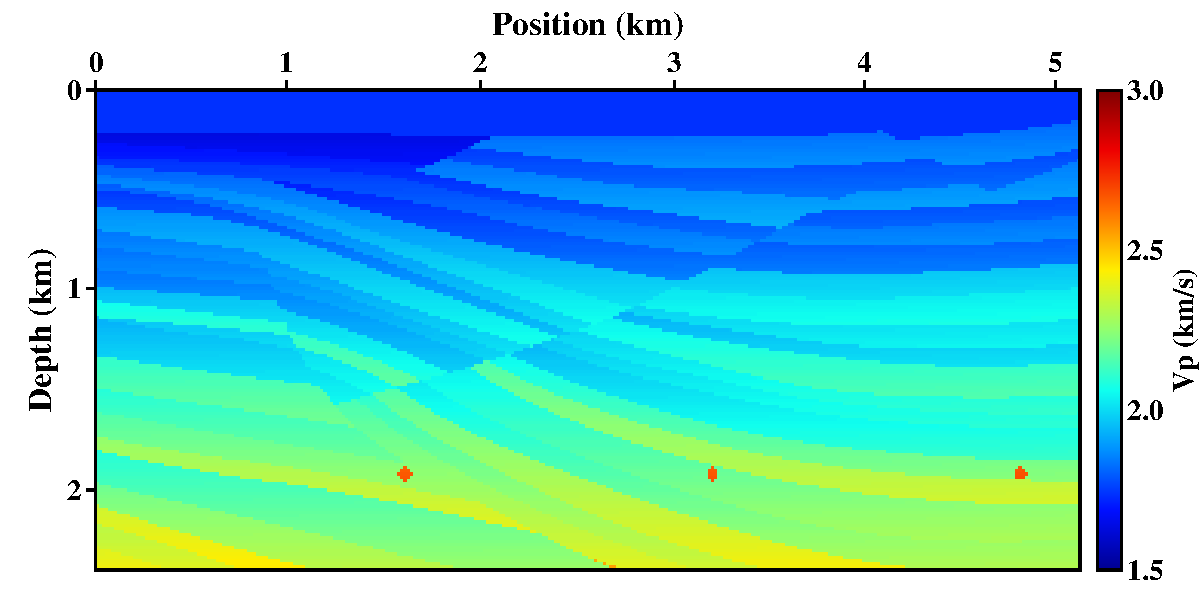
\includegraphics[width=0.48\textwidth]{Figure/chapter03/sigbee2/Fig/cuttruevp.pdf}}
   \subfloat[]{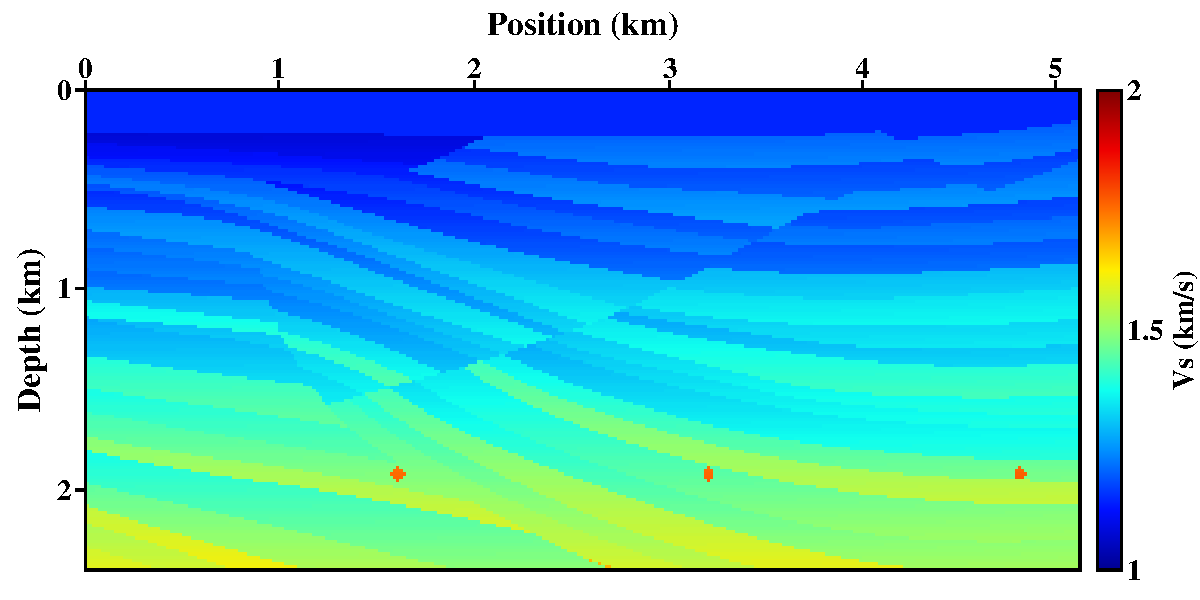
\includegraphics[width=0.48\textwidth]{Figure/chapter03/sigbee2/Fig/cuttruevs.pdf}}\\
   \subfloat[]{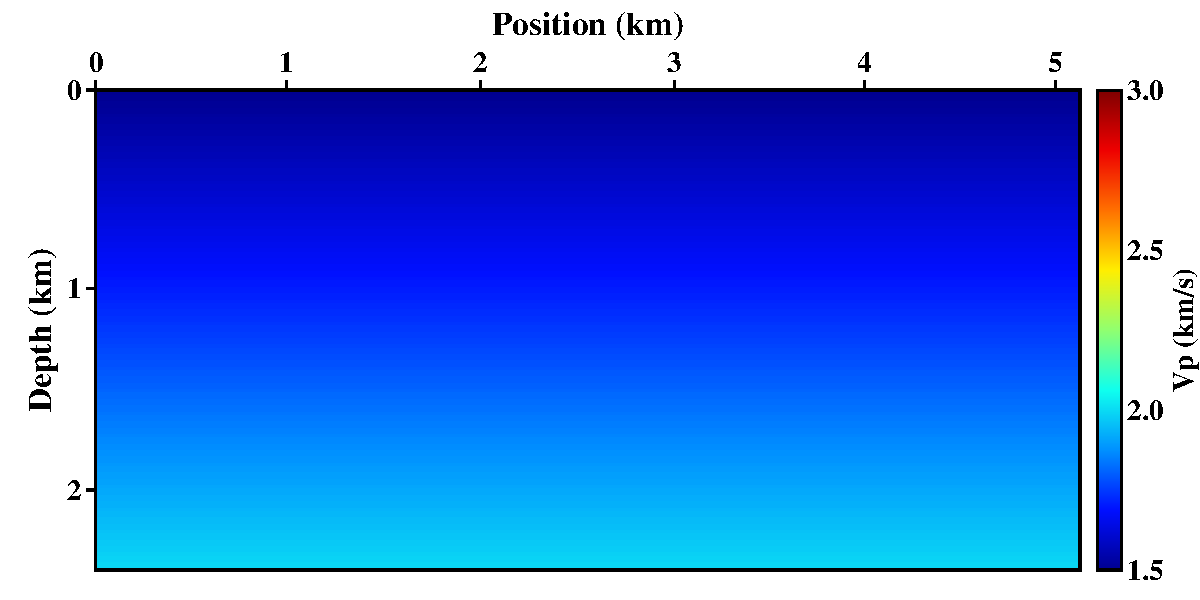
\includegraphics[width=0.48\textwidth]{Figure/chapter03/sigbee2/Fig/cutinitvp.pdf}}
   \subfloat[]{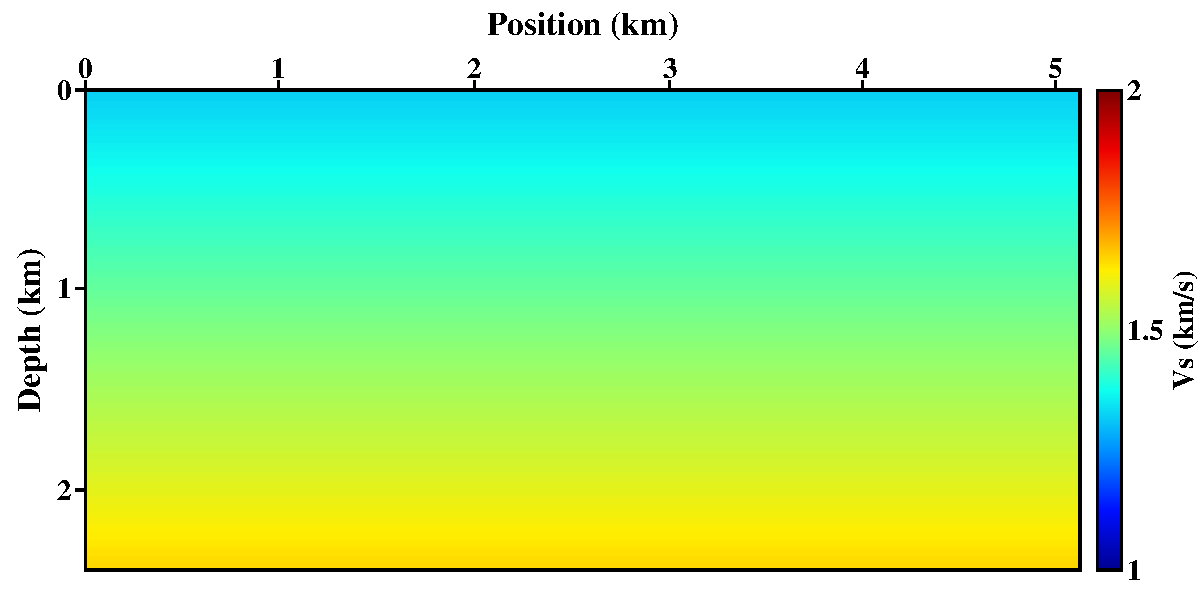
\includegraphics[width=0.48\textwidth]{Figure/chapter03/sigbee2/Fig/cutinitvs.pdf}}
   \caption{Sigbee2A model example. On the top are true models of 
   $V_p$ (a) and $V_s$ (b). On the bottom are initial models of $V_p$ (c) and $V_s$
   (d) linearly increasing with depth. }
   \label{fig:TrueAndInitial}
\end{figure}
我们采用Sigsbee2A模型的一部分来进行实验(如图\ref{fig:TrueAndInitial}a和\ref{fig:TrueAndInitial}b)。$V_s$模型通过一个固定的泊松比来产生。图\ref{fig:TrueAndInitial}c和\ref{fig:TrueAndInitial}d展示了$V_p$和$V_s$的初始模型,其速度值随深度线性增加。我们可以看到初始模型中,$V_p$比真实值偏低而$V_s$则偏高,
但这两者都偏离真实值很远。36炮地面模拟数据均匀的分布在地表,最大偏移距为4km,其震源为主频15Hz的纯P波震源。
\begin{figure}[!htb]
   \centering
   \subfloat[]{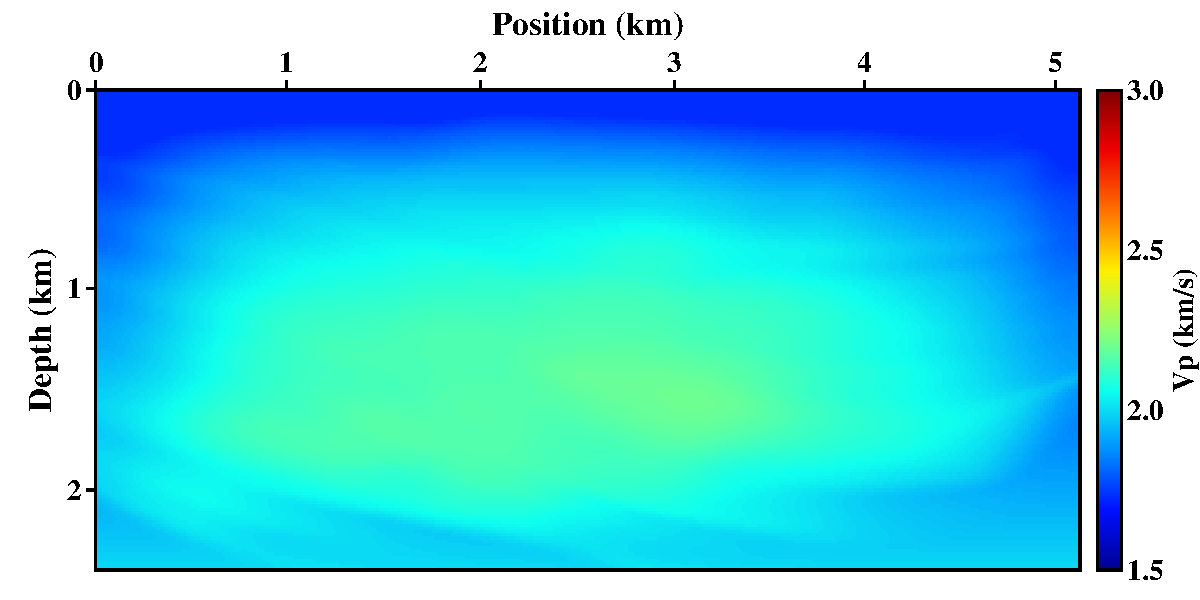
\includegraphics[width=0.48\textwidth]{Figure/chapter03/sigbee2/Fig/newinit3vp.pdf}}
   \subfloat[]{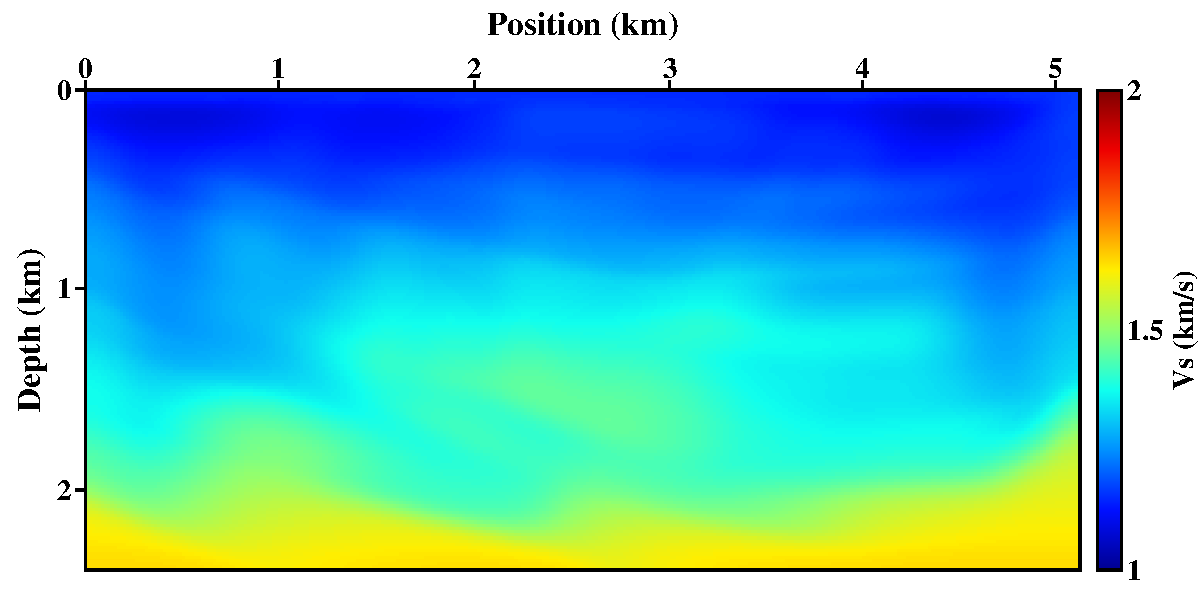
\includegraphics[width=0.48\textwidth]{Figure/chapter03/sigbee2/Fig/newinit3vs.pdf}}\\
   \subfloat[]{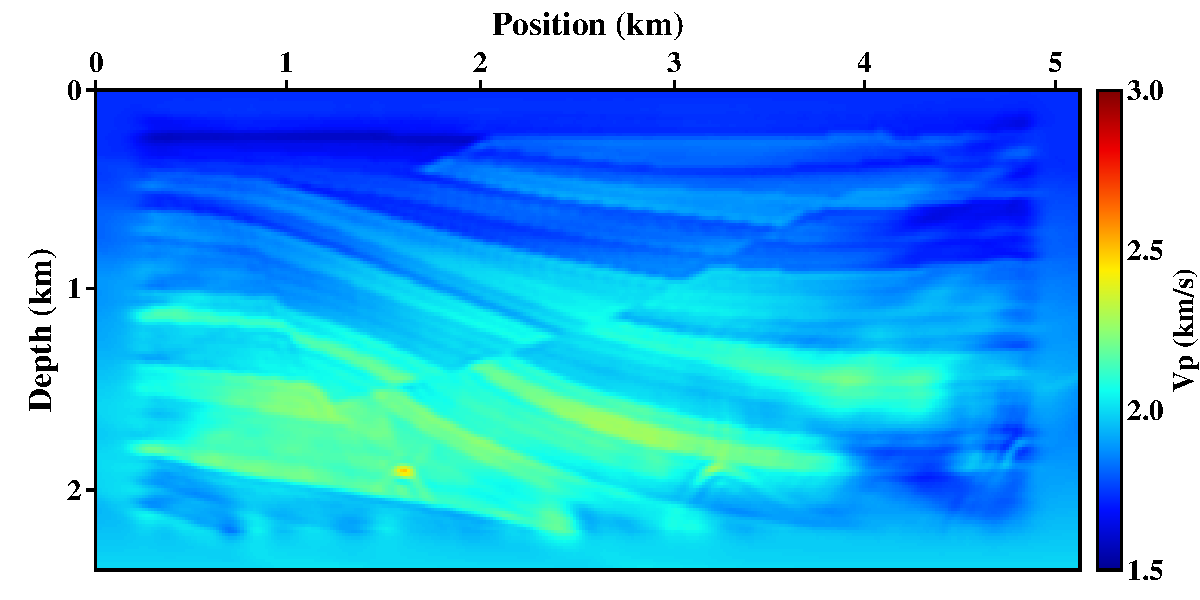
\includegraphics[width=0.48\textwidth]{Figure/chapter03/sigbee2/Fig/nodevp.pdf}}
   \subfloat[]{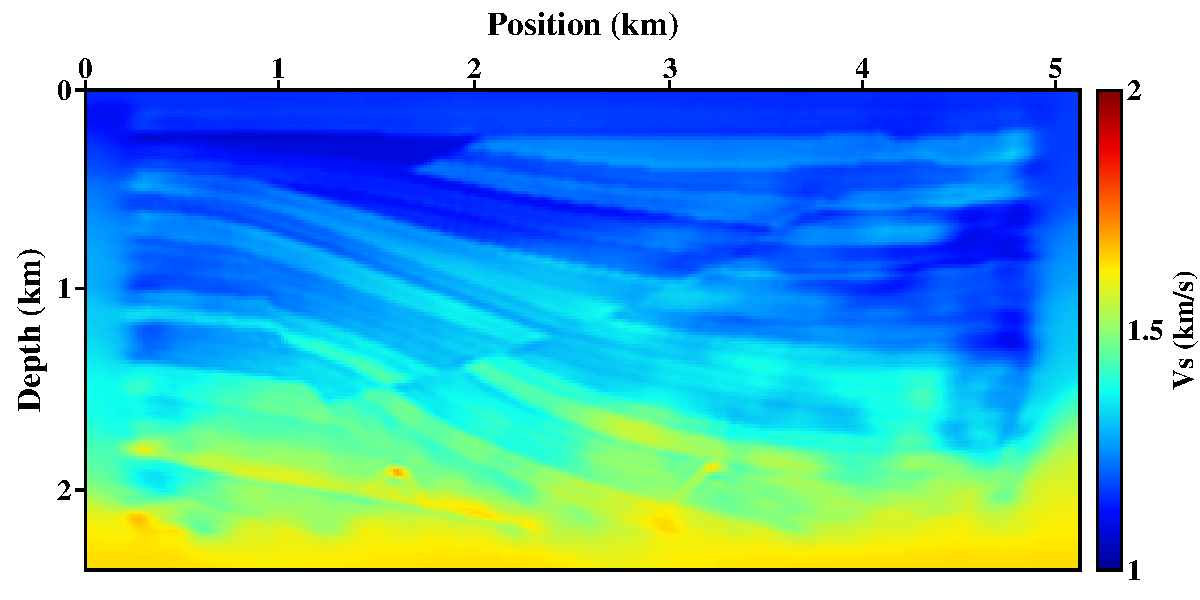
\includegraphics[width=0.48\textwidth]{Figure/chapter03/sigbee2/Fig/nodevs.pdf}}
   \caption{Inverted results of WERTI and EFWI. (a) and (b) are inverted $V_p$ and
       $V_s$ model through two-stage elastic WERTI with the linearly increased models
       as initial models. (c) and (d) are inverted $V_p$ and $V_s$ through EFWI using
   (a) and (b) as starting models.}
   \label{fig:InvertedModel}
\end{figure}
\begin{figure}[!htb]
   \centering
   \subfloat[]{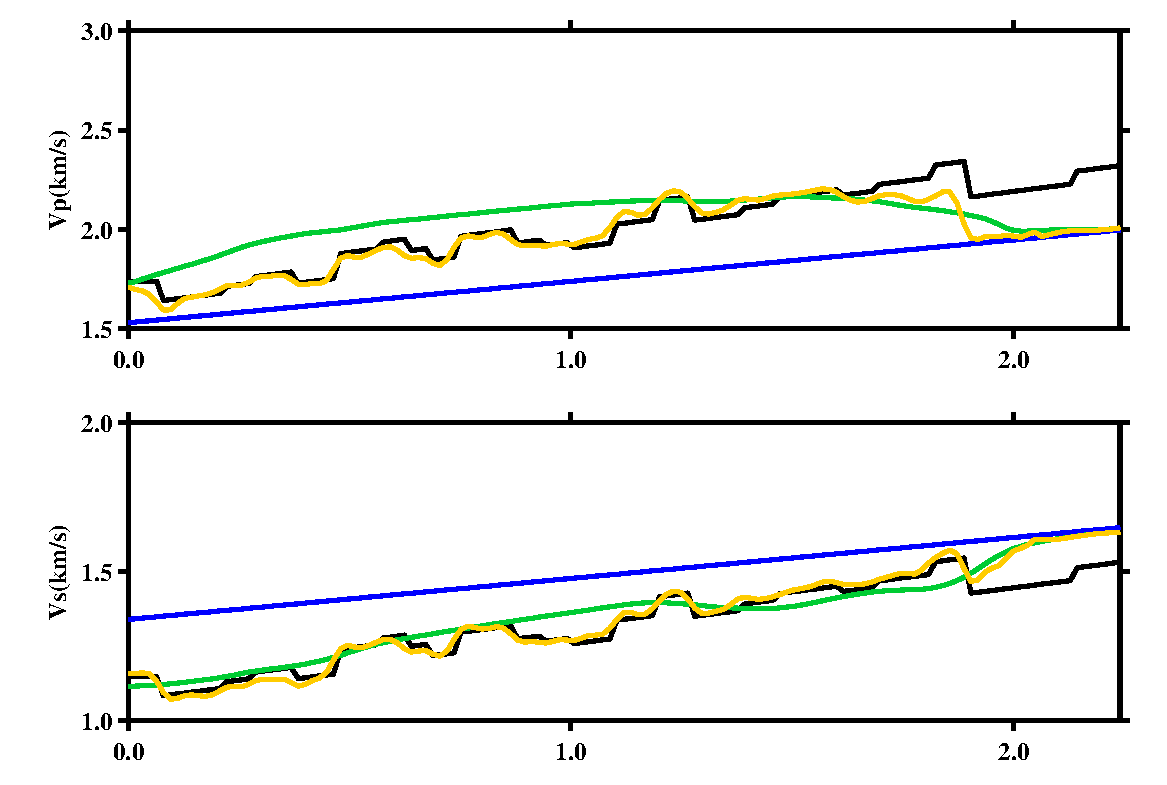
\includegraphics[width=0.48\textwidth]{Figure/chapter03/sigbee2/Fig/1km.pdf}}
   \subfloat[]{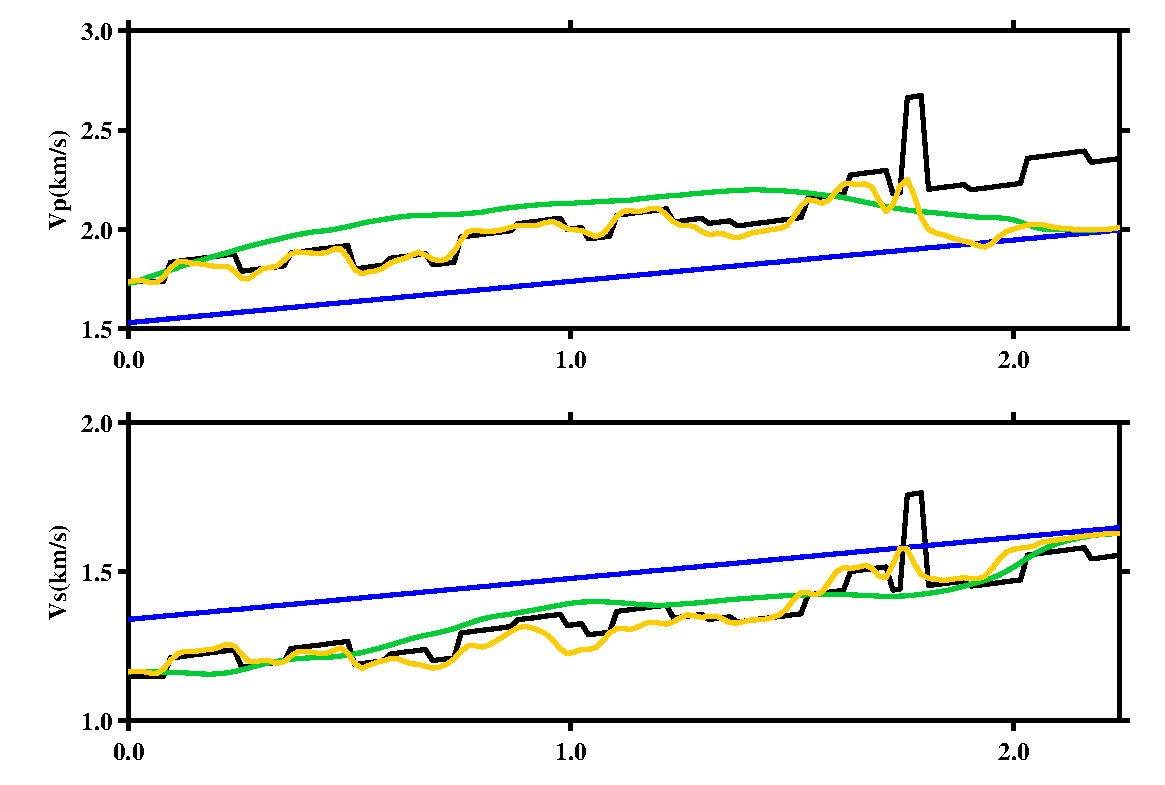
\includegraphics[width=0.48\textwidth]{Figure/chapter03/sigbee2/Fig/3km.pdf}}
   \caption{Vertical profiles of elastic WERTI and EFWI results at 1.4km (a) and
       3km (b). The black and blue lines indicate the true and linearly increased
       initial model. The green and yellow lines indicate the WERTI and EFWI results,
       respectively.
   }
   \label{fig:Profiles}
\end{figure}

图\ref{fig:InvertedModel}a和\ref{fig:InvertedModel}b为弹性WERTI的反演结果。由于线性增加的初始模型偏离真值很远,如果用该模型来进行常规EFWI,将不可避免的
受困于cycle-skipping问题。然而,经过每个阶段40次迭代之后,WERTI可以得到$V_p$和$V_s$较好的背景速度更新。采用WERTI的反演结果作为初始模型,我们重新进行了
常规EFWI反演。如图\ref{fig:InvertedModel}c和\ref{fig:InvertedModel}d所示,$V_p$和$V_s$模型都得到了很好的重建,除了模型右侧一小部分。原因可能是在
地面观测下,模型右侧的反射波覆盖不够导致WERTI不能准确的恢复该区域速度的长波长分量。图\ref{fig:Profiles}也展示了1.5km和3km处的垂向剖面。从图中可以看出,
弹性WERTI能够提供可靠的包含长波长分量的初始模型,并且以此为始模型的EFWI反演结果也与真实值很好的吻合。
